% Created by tikzDevice version 0.10.1 on 2017-11-06 20:32:13
% !TEX encoding = UTF-8 Unicode
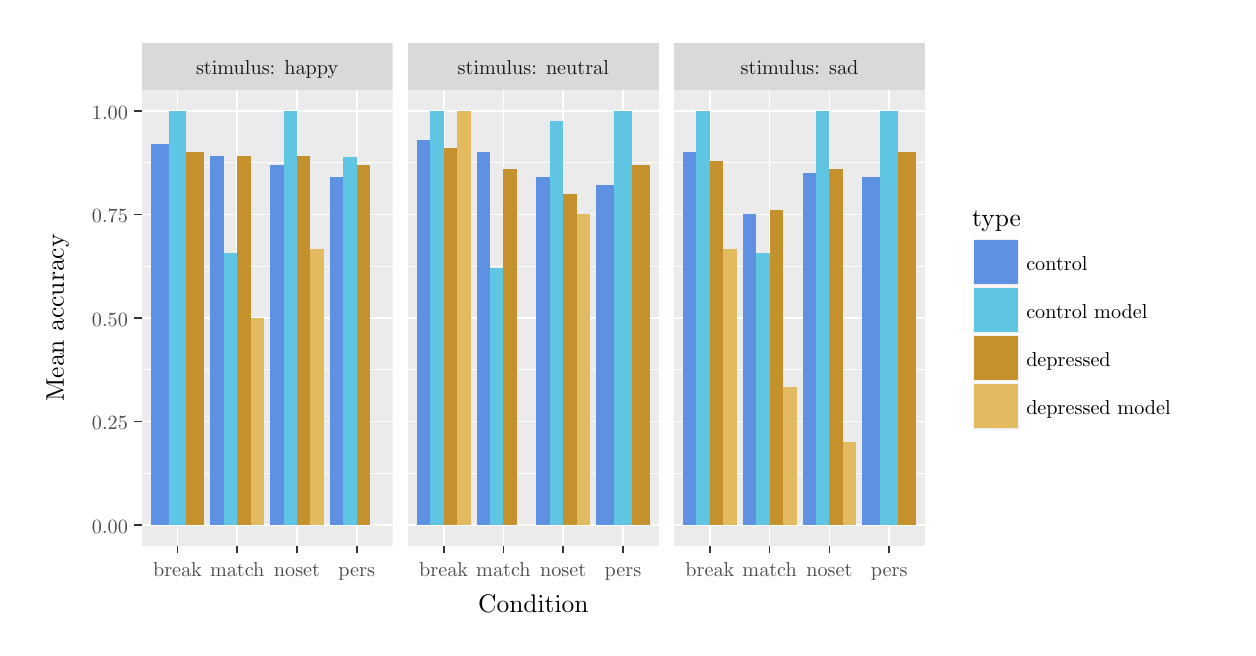
\begin{tikzpicture}[x=1pt,y=1pt]
\definecolor{fillColor}{RGB}{255,255,255}
\path[use as bounding box,fill=fillColor,fill opacity=0.00] (0,0) rectangle (433.62,216.81);
\begin{scope}
\path[clip] (  0.00,  0.00) rectangle (433.62,216.81);
\definecolor{drawColor}{RGB}{255,255,255}
\definecolor{fillColor}{RGB}{255,255,255}

\path[draw=drawColor,line width= 0.6pt,line join=round,line cap=round,fill=fillColor] (  0.00,  0.00) rectangle (433.62,216.81);
\end{scope}
\begin{scope}
\path[clip] ( 41.17, 29.59) rectangle (131.87,194.25);
\definecolor{fillColor}{gray}{0.92}

\path[fill=fillColor] ( 41.17, 29.59) rectangle (131.87,194.25);
\definecolor{drawColor}{RGB}{255,255,255}

\path[draw=drawColor,line width= 0.3pt,line join=round] ( 41.17, 55.78) --
	(131.87, 55.78);

\path[draw=drawColor,line width= 0.3pt,line join=round] ( 41.17, 93.21) --
	(131.87, 93.21);

\path[draw=drawColor,line width= 0.3pt,line join=round] ( 41.17,130.63) --
	(131.87,130.63);

\path[draw=drawColor,line width= 0.3pt,line join=round] ( 41.17,168.05) --
	(131.87,168.05);

\path[draw=drawColor,line width= 0.6pt,line join=round] ( 41.17, 37.07) --
	(131.87, 37.07);

\path[draw=drawColor,line width= 0.6pt,line join=round] ( 41.17, 74.49) --
	(131.87, 74.49);

\path[draw=drawColor,line width= 0.6pt,line join=round] ( 41.17,111.92) --
	(131.87,111.92);

\path[draw=drawColor,line width= 0.6pt,line join=round] ( 41.17,149.34) --
	(131.87,149.34);

\path[draw=drawColor,line width= 0.6pt,line join=round] ( 41.17,186.76) --
	(131.87,186.76);

\path[draw=drawColor,line width= 0.6pt,line join=round] ( 54.13, 29.59) --
	( 54.13,194.25);

\path[draw=drawColor,line width= 0.6pt,line join=round] ( 75.72, 29.59) --
	( 75.72,194.25);

\path[draw=drawColor,line width= 0.6pt,line join=round] ( 97.32, 29.59) --
	( 97.32,194.25);

\path[draw=drawColor,line width= 0.6pt,line join=round] (118.91, 29.59) --
	(118.91,194.25);
\definecolor{fillColor}{RGB}{196,145,45}

\path[fill=fillColor] ( 57.37, 37.07) rectangle ( 63.85,171.80);
\definecolor{fillColor}{RGB}{95,197,226}

\path[fill=fillColor] ( 50.89, 37.07) rectangle ( 57.37,186.76);
\definecolor{fillColor}{RGB}{95,145,226}

\path[fill=fillColor] ( 44.41, 37.07) rectangle ( 50.89,174.79);
\definecolor{fillColor}{RGB}{226,186,95}

\path[fill=fillColor] ( 80.58, 37.07) rectangle ( 85.44,111.92);
\definecolor{fillColor}{RGB}{196,145,45}

\path[fill=fillColor] ( 75.72, 37.07) rectangle ( 80.58,170.30);
\definecolor{fillColor}{RGB}{95,197,226}

\path[fill=fillColor] ( 70.86, 37.07) rectangle ( 75.72,135.44);
\definecolor{fillColor}{RGB}{95,145,226}

\path[fill=fillColor] ( 66.01, 37.07) rectangle ( 70.86,170.30);
\definecolor{fillColor}{RGB}{226,186,95}

\path[fill=fillColor] (102.18, 37.07) rectangle (107.03,136.87);
\definecolor{fillColor}{RGB}{196,145,45}

\path[fill=fillColor] ( 97.32, 37.07) rectangle (102.18,170.30);
\definecolor{fillColor}{RGB}{95,197,226}

\path[fill=fillColor] ( 92.46, 37.07) rectangle ( 97.32,186.76);
\definecolor{fillColor}{RGB}{95,145,226}

\path[fill=fillColor] ( 87.60, 37.07) rectangle ( 92.46,167.30);
\definecolor{fillColor}{RGB}{226,186,95}

\path[fill=fillColor] (123.77, 37.07) rectangle (128.63, 37.07);
\definecolor{fillColor}{RGB}{196,145,45}

\path[fill=fillColor] (118.91, 37.07) rectangle (123.77,167.30);
\definecolor{fillColor}{RGB}{95,197,226}

\path[fill=fillColor] (114.05, 37.07) rectangle (118.91,170.13);
\definecolor{fillColor}{RGB}{95,145,226}

\path[fill=fillColor] (109.19, 37.07) rectangle (114.05,162.81);
\end{scope}
\begin{scope}
\path[clip] (137.37, 29.59) rectangle (228.06,194.25);
\definecolor{fillColor}{gray}{0.92}

\path[fill=fillColor] (137.37, 29.59) rectangle (228.06,194.25);
\definecolor{drawColor}{RGB}{255,255,255}

\path[draw=drawColor,line width= 0.3pt,line join=round] (137.37, 55.78) --
	(228.06, 55.78);

\path[draw=drawColor,line width= 0.3pt,line join=round] (137.37, 93.21) --
	(228.06, 93.21);

\path[draw=drawColor,line width= 0.3pt,line join=round] (137.37,130.63) --
	(228.06,130.63);

\path[draw=drawColor,line width= 0.3pt,line join=round] (137.37,168.05) --
	(228.06,168.05);

\path[draw=drawColor,line width= 0.6pt,line join=round] (137.37, 37.07) --
	(228.06, 37.07);

\path[draw=drawColor,line width= 0.6pt,line join=round] (137.37, 74.49) --
	(228.06, 74.49);

\path[draw=drawColor,line width= 0.6pt,line join=round] (137.37,111.92) --
	(228.06,111.92);

\path[draw=drawColor,line width= 0.6pt,line join=round] (137.37,149.34) --
	(228.06,149.34);

\path[draw=drawColor,line width= 0.6pt,line join=round] (137.37,186.76) --
	(228.06,186.76);

\path[draw=drawColor,line width= 0.6pt,line join=round] (150.32, 29.59) --
	(150.32,194.25);

\path[draw=drawColor,line width= 0.6pt,line join=round] (171.92, 29.59) --
	(171.92,194.25);

\path[draw=drawColor,line width= 0.6pt,line join=round] (193.51, 29.59) --
	(193.51,194.25);

\path[draw=drawColor,line width= 0.6pt,line join=round] (215.10, 29.59) --
	(215.10,194.25);
\definecolor{fillColor}{RGB}{226,186,95}

\path[fill=fillColor] (155.18, 37.07) rectangle (160.04,186.76);
\definecolor{fillColor}{RGB}{196,145,45}

\path[fill=fillColor] (150.32, 37.07) rectangle (155.18,173.29);
\definecolor{fillColor}{RGB}{95,197,226}

\path[fill=fillColor] (145.46, 37.07) rectangle (150.32,186.76);
\definecolor{fillColor}{RGB}{95,145,226}

\path[fill=fillColor] (140.61, 37.07) rectangle (145.46,176.29);
\definecolor{fillColor}{RGB}{226,186,95}

\path[fill=fillColor] (176.77, 37.07) rectangle (181.63, 37.07);
\definecolor{fillColor}{RGB}{196,145,45}

\path[fill=fillColor] (171.92, 37.07) rectangle (176.77,165.81);
\definecolor{fillColor}{RGB}{95,197,226}

\path[fill=fillColor] (167.06, 37.07) rectangle (171.92,129.98);
\definecolor{fillColor}{RGB}{95,145,226}

\path[fill=fillColor] (162.20, 37.07) rectangle (167.06,171.80);
\definecolor{fillColor}{RGB}{226,186,95}

\path[fill=fillColor] (198.37, 37.07) rectangle (203.23,149.34);
\definecolor{fillColor}{RGB}{196,145,45}

\path[fill=fillColor] (193.51, 37.07) rectangle (198.37,156.83);
\definecolor{fillColor}{RGB}{95,197,226}

\path[fill=fillColor] (188.65, 37.07) rectangle (193.51,183.11);
\definecolor{fillColor}{RGB}{95,145,226}

\path[fill=fillColor] (183.79, 37.07) rectangle (188.65,162.81);
\definecolor{fillColor}{RGB}{196,145,45}

\path[fill=fillColor] (218.34, 37.07) rectangle (224.82,167.30);
\definecolor{fillColor}{RGB}{95,197,226}

\path[fill=fillColor] (211.86, 37.07) rectangle (218.34,186.76);
\definecolor{fillColor}{RGB}{95,145,226}

\path[fill=fillColor] (205.39, 37.07) rectangle (211.86,159.82);
\end{scope}
\begin{scope}
\path[clip] (233.56, 29.59) rectangle (324.25,194.25);
\definecolor{fillColor}{gray}{0.92}

\path[fill=fillColor] (233.56, 29.59) rectangle (324.25,194.25);
\definecolor{drawColor}{RGB}{255,255,255}

\path[draw=drawColor,line width= 0.3pt,line join=round] (233.56, 55.78) --
	(324.25, 55.78);

\path[draw=drawColor,line width= 0.3pt,line join=round] (233.56, 93.21) --
	(324.25, 93.21);

\path[draw=drawColor,line width= 0.3pt,line join=round] (233.56,130.63) --
	(324.25,130.63);

\path[draw=drawColor,line width= 0.3pt,line join=round] (233.56,168.05) --
	(324.25,168.05);

\path[draw=drawColor,line width= 0.6pt,line join=round] (233.56, 37.07) --
	(324.25, 37.07);

\path[draw=drawColor,line width= 0.6pt,line join=round] (233.56, 74.49) --
	(324.25, 74.49);

\path[draw=drawColor,line width= 0.6pt,line join=round] (233.56,111.92) --
	(324.25,111.92);

\path[draw=drawColor,line width= 0.6pt,line join=round] (233.56,149.34) --
	(324.25,149.34);

\path[draw=drawColor,line width= 0.6pt,line join=round] (233.56,186.76) --
	(324.25,186.76);

\path[draw=drawColor,line width= 0.6pt,line join=round] (246.52, 29.59) --
	(246.52,194.25);

\path[draw=drawColor,line width= 0.6pt,line join=round] (268.11, 29.59) --
	(268.11,194.25);

\path[draw=drawColor,line width= 0.6pt,line join=round] (289.70, 29.59) --
	(289.70,194.25);

\path[draw=drawColor,line width= 0.6pt,line join=round] (311.30, 29.59) --
	(311.30,194.25);
\definecolor{fillColor}{RGB}{226,186,95}

\path[fill=fillColor] (251.37, 37.07) rectangle (256.23,136.87);
\definecolor{fillColor}{RGB}{196,145,45}

\path[fill=fillColor] (246.52, 37.07) rectangle (251.37,168.80);
\definecolor{fillColor}{RGB}{95,197,226}

\path[fill=fillColor] (241.66, 37.07) rectangle (246.52,186.76);
\definecolor{fillColor}{RGB}{95,145,226}

\path[fill=fillColor] (236.80, 37.07) rectangle (241.66,171.80);
\definecolor{fillColor}{RGB}{226,186,95}

\path[fill=fillColor] (272.97, 37.07) rectangle (277.83, 86.97);
\definecolor{fillColor}{RGB}{196,145,45}

\path[fill=fillColor] (268.11, 37.07) rectangle (272.97,150.84);
\definecolor{fillColor}{RGB}{95,197,226}

\path[fill=fillColor] (263.25, 37.07) rectangle (268.11,135.44);
\definecolor{fillColor}{RGB}{95,145,226}

\path[fill=fillColor] (258.39, 37.07) rectangle (263.25,149.34);
\definecolor{fillColor}{RGB}{226,186,95}

\path[fill=fillColor] (294.56, 37.07) rectangle (299.42, 67.01);
\definecolor{fillColor}{RGB}{196,145,45}

\path[fill=fillColor] (289.70, 37.07) rectangle (294.56,165.81);
\definecolor{fillColor}{RGB}{95,197,226}

\path[fill=fillColor] (284.84, 37.07) rectangle (289.70,186.76);
\definecolor{fillColor}{RGB}{95,145,226}

\path[fill=fillColor] (279.99, 37.07) rectangle (284.84,164.31);
\definecolor{fillColor}{RGB}{196,145,45}

\path[fill=fillColor] (314.54, 37.07) rectangle (321.01,171.80);
\definecolor{fillColor}{RGB}{95,197,226}

\path[fill=fillColor] (308.06, 37.07) rectangle (314.54,186.76);
\definecolor{fillColor}{RGB}{95,145,226}

\path[fill=fillColor] (301.58, 37.07) rectangle (308.06,162.81);
\end{scope}
\begin{scope}
\path[clip] ( 41.17,194.25) rectangle (131.87,211.31);
\definecolor{fillColor}{gray}{0.85}

\path[fill=fillColor] ( 41.17,194.25) rectangle (131.87,211.31);
\definecolor{drawColor}{gray}{0.10}

\node[text=drawColor,anchor=base,inner sep=0pt, outer sep=0pt, scale=  0.73] at ( 86.52,199.75) {stimulus: happy};
\end{scope}
\begin{scope}
\path[clip] (137.37,194.25) rectangle (228.06,211.31);
\definecolor{fillColor}{gray}{0.85}

\path[fill=fillColor] (137.37,194.25) rectangle (228.06,211.31);
\definecolor{drawColor}{gray}{0.10}

\node[text=drawColor,anchor=base,inner sep=0pt, outer sep=0pt, scale=  0.73] at (182.71,199.75) {stimulus: neutral};
\end{scope}
\begin{scope}
\path[clip] (233.56,194.25) rectangle (324.25,211.31);
\definecolor{fillColor}{gray}{0.85}

\path[fill=fillColor] (233.56,194.25) rectangle (324.25,211.31);
\definecolor{drawColor}{gray}{0.10}

\node[text=drawColor,anchor=base,inner sep=0pt, outer sep=0pt, scale=  0.73] at (278.91,199.75) {stimulus: sad};
\end{scope}
\begin{scope}
\path[clip] (  0.00,  0.00) rectangle (433.62,216.81);
\definecolor{drawColor}{gray}{0.20}

\path[draw=drawColor,line width= 0.6pt,line join=round] ( 54.13, 26.84) --
	( 54.13, 29.59);

\path[draw=drawColor,line width= 0.6pt,line join=round] ( 75.72, 26.84) --
	( 75.72, 29.59);

\path[draw=drawColor,line width= 0.6pt,line join=round] ( 97.32, 26.84) --
	( 97.32, 29.59);

\path[draw=drawColor,line width= 0.6pt,line join=round] (118.91, 26.84) --
	(118.91, 29.59);
\end{scope}
\begin{scope}
\path[clip] (  0.00,  0.00) rectangle (433.62,216.81);
\definecolor{drawColor}{gray}{0.30}

\node[text=drawColor,anchor=base,inner sep=0pt, outer sep=0pt, scale=  0.73] at ( 54.13, 18.58) {break};

\node[text=drawColor,anchor=base,inner sep=0pt, outer sep=0pt, scale=  0.73] at ( 75.72, 18.58) {match};

\node[text=drawColor,anchor=base,inner sep=0pt, outer sep=0pt, scale=  0.73] at ( 97.32, 18.58) {noset};

\node[text=drawColor,anchor=base,inner sep=0pt, outer sep=0pt, scale=  0.73] at (118.91, 18.58) {pers};
\end{scope}
\begin{scope}
\path[clip] (  0.00,  0.00) rectangle (433.62,216.81);
\definecolor{drawColor}{gray}{0.20}

\path[draw=drawColor,line width= 0.6pt,line join=round] (150.32, 26.84) --
	(150.32, 29.59);

\path[draw=drawColor,line width= 0.6pt,line join=round] (171.92, 26.84) --
	(171.92, 29.59);

\path[draw=drawColor,line width= 0.6pt,line join=round] (193.51, 26.84) --
	(193.51, 29.59);

\path[draw=drawColor,line width= 0.6pt,line join=round] (215.10, 26.84) --
	(215.10, 29.59);
\end{scope}
\begin{scope}
\path[clip] (  0.00,  0.00) rectangle (433.62,216.81);
\definecolor{drawColor}{gray}{0.30}

\node[text=drawColor,anchor=base,inner sep=0pt, outer sep=0pt, scale=  0.73] at (150.32, 18.58) {break};

\node[text=drawColor,anchor=base,inner sep=0pt, outer sep=0pt, scale=  0.73] at (171.92, 18.58) {match};

\node[text=drawColor,anchor=base,inner sep=0pt, outer sep=0pt, scale=  0.73] at (193.51, 18.58) {noset};

\node[text=drawColor,anchor=base,inner sep=0pt, outer sep=0pt, scale=  0.73] at (215.10, 18.58) {pers};
\end{scope}
\begin{scope}
\path[clip] (  0.00,  0.00) rectangle (433.62,216.81);
\definecolor{drawColor}{gray}{0.20}

\path[draw=drawColor,line width= 0.6pt,line join=round] (246.52, 26.84) --
	(246.52, 29.59);

\path[draw=drawColor,line width= 0.6pt,line join=round] (268.11, 26.84) --
	(268.11, 29.59);

\path[draw=drawColor,line width= 0.6pt,line join=round] (289.70, 26.84) --
	(289.70, 29.59);

\path[draw=drawColor,line width= 0.6pt,line join=round] (311.30, 26.84) --
	(311.30, 29.59);
\end{scope}
\begin{scope}
\path[clip] (  0.00,  0.00) rectangle (433.62,216.81);
\definecolor{drawColor}{gray}{0.30}

\node[text=drawColor,anchor=base,inner sep=0pt, outer sep=0pt, scale=  0.73] at (246.52, 18.58) {break};

\node[text=drawColor,anchor=base,inner sep=0pt, outer sep=0pt, scale=  0.73] at (268.11, 18.58) {match};

\node[text=drawColor,anchor=base,inner sep=0pt, outer sep=0pt, scale=  0.73] at (289.70, 18.58) {noset};

\node[text=drawColor,anchor=base,inner sep=0pt, outer sep=0pt, scale=  0.73] at (311.30, 18.58) {pers};
\end{scope}
\begin{scope}
\path[clip] (  0.00,  0.00) rectangle (433.62,216.81);
\definecolor{drawColor}{gray}{0.30}

\node[text=drawColor,anchor=base east,inner sep=0pt, outer sep=0pt, scale=  0.73] at ( 36.22, 34.04) {0.00};

\node[text=drawColor,anchor=base east,inner sep=0pt, outer sep=0pt, scale=  0.73] at ( 36.22, 71.46) {0.25};

\node[text=drawColor,anchor=base east,inner sep=0pt, outer sep=0pt, scale=  0.73] at ( 36.22,108.89) {0.50};

\node[text=drawColor,anchor=base east,inner sep=0pt, outer sep=0pt, scale=  0.73] at ( 36.22,146.31) {0.75};

\node[text=drawColor,anchor=base east,inner sep=0pt, outer sep=0pt, scale=  0.73] at ( 36.22,183.73) {1.00};
\end{scope}
\begin{scope}
\path[clip] (  0.00,  0.00) rectangle (433.62,216.81);
\definecolor{drawColor}{gray}{0.20}

\path[draw=drawColor,line width= 0.6pt,line join=round] ( 38.42, 37.07) --
	( 41.17, 37.07);

\path[draw=drawColor,line width= 0.6pt,line join=round] ( 38.42, 74.49) --
	( 41.17, 74.49);

\path[draw=drawColor,line width= 0.6pt,line join=round] ( 38.42,111.92) --
	( 41.17,111.92);

\path[draw=drawColor,line width= 0.6pt,line join=round] ( 38.42,149.34) --
	( 41.17,149.34);

\path[draw=drawColor,line width= 0.6pt,line join=round] ( 38.42,186.76) --
	( 41.17,186.76);
\end{scope}
\begin{scope}
\path[clip] (  0.00,  0.00) rectangle (433.62,216.81);
\definecolor{drawColor}{RGB}{0,0,0}

\node[text=drawColor,anchor=base,inner sep=0pt, outer sep=0pt, scale=  0.92] at (182.71,  5.50) {Condition};
\end{scope}
\begin{scope}
\path[clip] (  0.00,  0.00) rectangle (433.62,216.81);
\definecolor{drawColor}{RGB}{0,0,0}

\node[text=drawColor,rotate= 90.00,anchor=base,inner sep=0pt, outer sep=0pt, scale=  0.92] at ( 13.08,111.92) {Mean accuracy};
\end{scope}
\begin{scope}
\path[clip] (  0.00,  0.00) rectangle (433.62,216.81);
\definecolor{fillColor}{RGB}{255,255,255}

\path[fill=fillColor] (335.63, 65.58) rectangle (428.12,158.25);
\end{scope}
\begin{scope}
\path[clip] (  0.00,  0.00) rectangle (433.62,216.81);
\definecolor{drawColor}{RGB}{0,0,0}

\node[text=drawColor,anchor=base west,inner sep=0pt, outer sep=0pt, scale=  0.92] at (341.32,144.99) {type};
\end{scope}
\begin{scope}
\path[clip] (  0.00,  0.00) rectangle (433.62,216.81);
\definecolor{drawColor}{RGB}{255,255,255}
\definecolor{fillColor}{gray}{0.95}

\path[draw=drawColor,line width= 0.6pt,line join=round,line cap=round,fill=fillColor] (341.32,123.31) rectangle (358.67,140.65);
\end{scope}
\begin{scope}
\path[clip] (  0.00,  0.00) rectangle (433.62,216.81);
\definecolor{fillColor}{RGB}{95,145,226}

\path[fill=fillColor] (342.04,124.02) rectangle (357.96,139.94);
\end{scope}
\begin{scope}
\path[clip] (  0.00,  0.00) rectangle (433.62,216.81);
\definecolor{drawColor}{RGB}{255,255,255}
\definecolor{fillColor}{gray}{0.95}

\path[draw=drawColor,line width= 0.6pt,line join=round,line cap=round,fill=fillColor] (341.32,105.96) rectangle (358.67,123.31);
\end{scope}
\begin{scope}
\path[clip] (  0.00,  0.00) rectangle (433.62,216.81);
\definecolor{fillColor}{RGB}{95,197,226}

\path[fill=fillColor] (342.04,106.67) rectangle (357.96,122.60);
\end{scope}
\begin{scope}
\path[clip] (  0.00,  0.00) rectangle (433.62,216.81);
\definecolor{drawColor}{RGB}{255,255,255}
\definecolor{fillColor}{gray}{0.95}

\path[draw=drawColor,line width= 0.6pt,line join=round,line cap=round,fill=fillColor] (341.32, 88.62) rectangle (358.67,105.96);
\end{scope}
\begin{scope}
\path[clip] (  0.00,  0.00) rectangle (433.62,216.81);
\definecolor{fillColor}{RGB}{196,145,45}

\path[fill=fillColor] (342.04, 89.33) rectangle (357.96,105.25);
\end{scope}
\begin{scope}
\path[clip] (  0.00,  0.00) rectangle (433.62,216.81);
\definecolor{drawColor}{RGB}{255,255,255}
\definecolor{fillColor}{gray}{0.95}

\path[draw=drawColor,line width= 0.6pt,line join=round,line cap=round,fill=fillColor] (341.32, 71.27) rectangle (358.67, 88.62);
\end{scope}
\begin{scope}
\path[clip] (  0.00,  0.00) rectangle (433.62,216.81);
\definecolor{fillColor}{RGB}{226,186,95}

\path[fill=fillColor] (342.04, 71.98) rectangle (357.96, 87.91);
\end{scope}
\begin{scope}
\path[clip] (  0.00,  0.00) rectangle (433.62,216.81);
\definecolor{drawColor}{RGB}{0,0,0}

\node[text=drawColor,anchor=base west,inner sep=0pt, outer sep=0pt, scale=  0.73] at (360.84,128.95) {control};
\end{scope}
\begin{scope}
\path[clip] (  0.00,  0.00) rectangle (433.62,216.81);
\definecolor{drawColor}{RGB}{0,0,0}

\node[text=drawColor,anchor=base west,inner sep=0pt, outer sep=0pt, scale=  0.73] at (360.84,111.60) {control model};
\end{scope}
\begin{scope}
\path[clip] (  0.00,  0.00) rectangle (433.62,216.81);
\definecolor{drawColor}{RGB}{0,0,0}

\node[text=drawColor,anchor=base west,inner sep=0pt, outer sep=0pt, scale=  0.73] at (360.84, 94.26) {depressed};
\end{scope}
\begin{scope}
\path[clip] (  0.00,  0.00) rectangle (433.62,216.81);
\definecolor{drawColor}{RGB}{0,0,0}

\node[text=drawColor,anchor=base west,inner sep=0pt, outer sep=0pt, scale=  0.73] at (360.84, 76.91) {depressed model};
\end{scope}
\end{tikzpicture}
